%%%%%%%%%%%%%%%%%%%%%%%%%%%%%%%%%%%%%%%%%
% Journal Article
% LaTeX Template
% Version 1.3 (9/9/13)
%
% This template has been downloaded from:
% http://www.LaTeXTemplates.com
%
% Original author:
% Frits Wenneker (http://www.howtotex.com)
%
% License:
% CC BY-NC-SA 3.0 (http://creativecommons.org/licenses/by-nc-sa/3.0/)
%
%%%%%%%%%%%%%%%%%%%%%%%%%%%%%%%%%%%%%%%%%

%----------------------------------------------------------------------------------------
%	PACKAGES AND OTHER DOCUMENT CONFIGURATIONS
%----------------------------------------------------------------------------------------

\documentclass{article}

\usepackage{mathtools} %tools for mathematical writing
\usepackage{caption}
\usepackage{subfig}
\usepackage{float}
\usepackage{color}
\usepackage{adjustbox}
\usepackage[toc,page]{appendix}

\usepackage[sc]{mathpazo} % Use the Palatino font
\usepackage[T1]{fontenc} % Use 8-bit encoding that has 256 glyphs
\linespread{1.05} % Line spacing - Palatino needs more space between lines
\usepackage{microtype} % Slightly tweak font spacing for aesthetics

\usepackage[hmarginratio=1:1,top=32mm,columnsep=20pt]{geometry} % Document margins
%\usepackage{multicol} % Used for the two-column layout of the document
%\usepackage[hang, small,labelfont=bf,up,textfont=it,up]{caption} % Custom captions under/above floats in tables or figures
\usepackage{booktabs} % Horizontal rules in tables
%\usepackage{float} % Required for tables and figures in the multi-column environment - they need to be placed in specific locations with the [H] (e.g. \begin{table}[H])
\usepackage{hyperref} % For hyperlinks in the PDF

\usepackage{lettrine} % The lettrine is the first enlarged letter at the beginning of the text
\usepackage{paralist} % Used for the compactitem environment which makes bullet points with less space between them

\usepackage{abstract} % Allows abstract customization
\renewcommand{\abstractnamefont}{\normalfont\bfseries} % Set the "Abstract" text to bold
\renewcommand{\abstracttextfont}{\normalfont\small\itshape} % Set the abstract itself to small italic text

\usepackage{titlesec} % Allows customization of titles
%\renewcommand\thesection{\Roman{section}} % Roman numerals for the sections
%\renewcommand\thesubsection{\Roman{subsection}} % Roman numerals for subsections
\titleformat{\section}[block]{\large\scshape\centering}{\thesection.}{1em}{} % Change the look of the section titles
\titleformat{\subsection}[block]{\large}{\thesubsection.}{1em}{} % Change the look of the section titles

\usepackage{fancyhdr} % Headers and footers
\pagestyle{fancy} % All pages have headers and footers
\fancyhead{} % Blank out the default header
\fancyfoot{} % Blank out the default footer
%\fancyhead[C]{Running title $\bullet$ November 2012 $\bullet$ Vol. XXI, No. 1} % Custom header text
\fancyfoot[RO,LE]{\thepage} % Custom footer text

\usepackage{algorithm}% http://ctan.org/pkg/algorithms
\usepackage{algpseudocode}% http://ctan.org/pkg/algorithmicx

\usepackage[acronym]{glossaries} %Used for the acronyms

\usepackage{tikz}	%Used for the drawings
\usetikzlibrary{arrows, calc,decorations.pathmorphing,positioning,decorations.markings}

\DeclarePairedDelimiter\ceil{\lceil}{\rceil}
\DeclarePairedDelimiter\floor{\lfloor}{\rfloor}

%My definitions
%\renewcommand{\tablename}{Table}

\newtheorem{theorem}{Theorem}
\newtheorem{proposition}{Proposition}[section]
\newtheorem{corollary}{Corollary}[theorem]
\newtheorem{remark}{Remark}
\newenvironment{proof}{\begin{trivlist} \item[]\textbf{Proof}
\hspace{0cm} }{\hfill $\Box$ \end{trivlist}}
\newtheorem{mydef}{Definition}[section]
%\newcommand{\eqref}[1]{\mbox{(\ref{#1})}}
\newcommand{\Tr}{\mbox{Tr}}

%Set space between paragraphs
\setlength{\parskip}{2ex}

\usepackage{authblk}
%----------------------------------------------------------------------------------------
%	TITLE SECTION
%----------------------------------------------------------------------------------------

\title{Problem statement and Data collection}
\author[1]{David Laredo\thanks{dlaredorazo@ucmerced.edu}}

\date{}
%\renewcommand\Authands{ and }

% Generate the glossary
%\makeglossaries
%\renewcommand*{\acronymname}{Acronyms}

%----------------------------------------------------------------------------------------

%----------------------------------------------------------------------------------------
%	FIGURE CONFIGURATION
%----------------------------------------------------------------------------------------
\tikzset{
    shadedrec/.style={
        rectangle,
        draw=black,
        top color=gray, 
        bottom color=white, 
        shading angle={135},
        text width=3cm,
        inner sep=1em,
        rounded corners=1.2ex,
        very thick,
        text centered},
    snake arrow/.style={
        decorate,
        decoration={zigzag,amplitude=3mm,segment length=5mm,post length=0mm}},
    damper/.style={
        very thick,
        decoration={markings,  
        mark connection node=dmp,
        mark=at position 0.5 with 
        {
            \node (dmp) [very thick,transform shape,text width=.3cm,rotate=-90,minimum height=3pt,draw=none, fill=black,outer xsep=2pt, outer ysep=1pt] {};
            \draw [very thick] ($(dmp.north east)+(-.6pt,0)$) -- ($(dmp.south east)+(-.6pt,0)$) -- ($(dmp.south west)+(-.6pt,0)$) -- ($(dmp.north west)+(-.6pt,0)$);
            \draw [very thick,rotate=-90] ($(dmp.north)+(0,-5pt)$) -- ($(dmp.north)+(0,5pt)$);
        }
    }, decorate}
}
%----------------------------------------------------------------------------------------

\makeglossaries
%Term definitions
\newacronym{moo}{MOO}{Multi-objective Optimization}
\newacronym{mop}{MOP}{Multi-objective Optimization Problem}
\newacronym{mmop}{MMOP}{Mixed-Integer Multi-objective Optimization Problem}
\newacronym{eds}{EDS}{Enhanced Directed Search}
\newacronym{dzz}{DZZ}{Direct Zig Zag}
\newacronym{nsga2}{NSGA-II}{Non-Sorted Genetic Algorithm II}
\newacronym{sop}{SOP}{Single-objective Optimization Problem}
\newacronym{pc}{PC}{Predictor-Corrector}
\newacronym{moea}{MOEA}{Multi-objective Optimization Evolutionary Algorithm}
\newacronym{ea}{EA}{Evolutionary Algorithm}
\newacronym{ds}{DS}{Directed Search}
\newacronym{kkt}{KKT}{Karush-Kuhn-Tucker}
\newacronym{bop}{BOP}{Bi-objective Optimization Problem}
\newacronym{gd}{GD}{Generational Distance}
\newacronym{igd}{IGD}{Inverted Generational Distance}
\newacronym{gsa}{GSA}{Gradient Subspace Approximation}
\newacronym{ift}{IFT}{Implicit Function Theorem}
\newacronym{fps}{FPS}{First Pareto Solution}
\newacronym{moead}{MOEA-D}{Multi-objective Optimization Evolutionary Algorithm based on Decomposition}
\newacronym{pf}{PF}{Pareto Front}
\newacronym{nbi}{NBI}{Normal Boundary Intersection}
\newacronym{pso}{PSO}{Particle Swarm Optimization} %Insert acronym list

\begin{document}

\maketitle % Insert title

\thispagestyle{fancy} % All pages have headers and footers

%Used to not expand the first acronym
\glsunsetall

%----------------------------------------------------------------------------------------
%	ABSTRACT
%----------------------------------------------------------------------------------------

\begin{abstract}

\noindent 

This report describes the procedure by which the data from SE2 \gls{hvac} system is obtained, stored and preprocessed. A database is designed to store all the information regarding the status of the \gls{hvac} system in SE2, this report also discuses its design and implementation.

\end{abstract}

%----------------------------------------------------------------------------------------
%	ARTICLE CONTENTS
%----------------------------------------------------------------------------------------

%Asymptotic Complexities of the Proposed Algorithms
%Computational Power of the available equipment
\section{Introduction}

This documents presents and describes the procedure by which the data from the SE 2 \gls{hvac} system is gathered and stored. A brief description of \gls{hvac} systems is given and a database model that will be used for storing the raw data coming from the sensors in the \gls{hvac} network is presented and discussed in detail. The report is organized as follows: In Section \ref{section:background} a brief discussion on how \gls{hvac} systems operate and how they are comprised is presented along with a brief review of some of the current fault detection methods used in \gls{hvac}. Section \ref{section:dataAcquisition} describes the BACnet protocol on how it is used to access the raw data from the sensors. Finally Section \ref{section:databaseDesign} describes in detail how the database was designed and what are its advantages over other approaches for storing the data.
\section{Background}
\label{section:background}

Heating, ventilation and air conditioning (\gls{hvac}) is a technology of indoor environmental comfort. It is usually implemented in large office, commercial and industrial buildings such as schools, airports, malls, factories, hospitals, etc. Its ultimate goal is to maintain thermal comfort and create healthy indoor air quality while keeping an affordable maintenance cost, being energy efficient and environmentally friendly.

Currently, \gls{hvac} is comprised of numerous components, advanced sensing technologies, advanced control algorithms and even artificial intelligence techniques, which have been introduced to help the system meet its operational objectives across different types of buildings worldwide. Hence \gls{hvac} systems are regarded as highly interdisciplinary and complex mechanical systems.

According to the U.S. Energy Information Administration, residential and commercial sectors account for $40\%$ of the total share of energy consumed in the United States in 2016 \cite{us_energy_usage}. Heating, ventilation and air conditioning make up almost $50\%$ of the total energy consumption \cite{residential_energy_use_us, commericial_energy_use_us}.

As with any other mechanical system, \gls{hvac} systems are prone to faults and as its scale and complexity increases the detection, identification and pinpointing of such faults within the \gls{hvac} network becomes a very challenging and hard to achieve task. Here, faults include not only complete equipment failures, but also non-optimal operating conditions, e.g., occupant discomfort, energy inefficiency, poor choice of operating targets, sensor calibration error, poor controller tuning, etc. Some common faults that an \gls{hvac} system may be prone to are: a stuck damper, stuck water valve, coolant leakage, airflow leakage (due to breaches in the ducts), fan malfunction, etc. Such failures may degrade the overall performance of the \gls{hvac} system and thus lead to energy waste. Therefore, it is of great potential to develop automatic, quick responding, intelligent, and reliable monitoring and diagnosis tools to ensure the normal operation of the system, increasing, as a direct consequence, its energy consumption efficiency.

According to the National Institute of Standards and Technology (\gls{nist}), Fault Detection and Diagnosis (\gls{fdd}) methods have a potential to save 10\%-40\% of \gls{hvac} energy consumption \cite{schein1}. \gls{fdd} tools for \gls{hvac} is therefore critical to increase the energy efficiency for buildings. Since the 1980s, researchers have been striving to improve the energy efficiency of the system due to rising energy costs and increased awareness of the environment.

\subsection{Fault Detection in \gls{hvac} systems}

As mentioned in the previous section, \gls{fdd} tools can help improve the overall energy consumption of and \gls{hvac} system by timely detecting, isolating (classifying) and pinpointing the location of the faults so that they can be fixed as soon as they are detected. Several methods have been proposed for achieving this goal. 

Fault Detection and Isolation (\gls{fdi}) is a subfield of control engineering concerned with monitoring a system, identifying when a fault has occurred, and pinpointing the type of fault and its location. Usually the methods and techniques for doing \gls{fdi} can be divided in two groups:

\begin{itemize}
\item A model based approach that measures the discrepancies between the actual sensor readings and the expected values derived from the model.
\item A pattern recognition approach that looks for patterns in the data that may indicate a fault.
\end{itemize}

In the first group some model of the system is used to decide about the occurrence of a fault. The model may be mathematical or knowledge based, here energy and thermal models have been used to successfully identify certain faults and tune the controllers as in \cite{wu_thesis, wei_thesis, model_fault_detection1}. In the second group some mathematical or statistical operations are performed to the measurements, this approach also considers machine learning algorithms that will look for patterns in the data which may be indicative of a fault. Such approaches have been specially considered in the domain of machine learning as in \cite{fault_detection_mechanical1, fault_diagnosis_ahu, cmeans_fault_detection, fault_diagnosis_refrigerant}.

In this work the pattern recognition approach is considered over the model based one, this will allow the system to detect, classify and locate faults within the system without specific knowledge of the network except for its topology.

\subsection{A generic \gls{hvac} system}

A generic \gls{hvac} is comprised of several components, among the most noticeable ones we can find are: the Air Handling Unit, the Variable Air Volume, the Staged Air Volume and the Thermafuser.  The Air Handling Unit (\gls{ahu}) is the main component of the \gls{hvac} network. The function of the \gls{ahu} is to regulate, condition and distribute the conditioned air to the other components of the system though  a ductwork ventilation system which is also used for returning air to the \gls{ahu}. \gls{ahu} is usually a large metal box containing inside fans, heating and/or cooling elements, filter racks or chambers, sound atenuators and dampers. Figure \ref{fig:ahu_inside} shows an inside view of how the majority of \gls{ahu}s are built, while Figure \ref{fig:ahu_inside} shows and outside view of an \gls{ahu}.

\begin{figure}[H]
	\centering
		\begin{minipage}{.5\textwidth}
 			 \centering
  			\includegraphics[width=55mm, height=45mm]{resources/AHUInside.png}
  			\caption{Inside view of \gls{ahu}}
  			%\captionof{figure}{A figure}
 			 \label{fig:ahu_inside}
		\end{minipage}%
		\begin{minipage}{.5\textwidth}
  			\centering
  			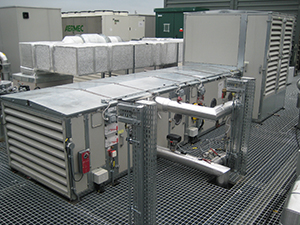
\includegraphics[width=55mm, height=45mm]{resources/AHUOutside.png}
  			\caption{Outside view of \gls{ahu}}
  			%\captionof{figure}{Another figure}
  			\label{fig:ahu_outside}
		\end{minipage}
\end{figure}

In the second level of the \gls{hvac} topology we have the Variable Air Volume (\gls{vav}) and the Staged Air Volume (\gls{sav}). The main goal of these two components is two vary the airflow and the temperature of the supply air to be further distributed, they achieve this goal by controlling the damper position at the entrance of the \gls{vav}/\gls{sav} and modifying the temperature by means of cooling and heating coils. Figure ... shows the inside composition of a generic \gls{vav} while Figure ... shows the inside composition for a generic \gls{sav}.

\begin{figure}[H]
	\centering
		\begin{minipage}{.5\textwidth}
 			 \centering
  			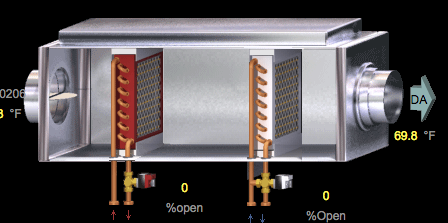
\includegraphics[width=55mm, height=45mm]{resources/VAVInside.png}
  			\caption{Inside view of a \gls{vav}}
  			%\captionof{figure}{A figure}
 			 \label{fig:vav_inside}
		\end{minipage}%
		\begin{minipage}{.5\textwidth}
  			\centering
  			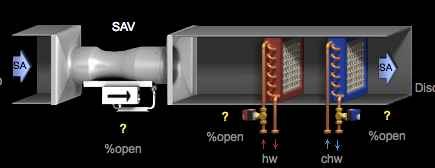
\includegraphics[width=55mm, height=45mm]{resources/SAVInside.png}
  			\caption{Outside view of a \gls{sav}}
  			%\captionof{figure}{Another figure}
  			\label{fig:sav_inside}
		\end{minipage}
\end{figure}

Finally, the last component in the chain are the Thermafusers, these components are where the air comes out into the room and their purpose is to regulate the airflow that comes into the room, it achieves this goal by using a set of dampers along its edges. Figure \ref{fig:thermafuser} shows a generic thermafuser mounted on the ceiling of a room.

\begin{figure}[H]
	\centering
  	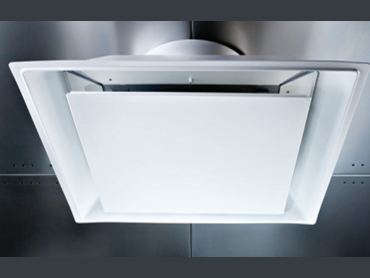
\includegraphics[width=55mm, height=45mm]{resources/thermafuser.png}
  	\caption{View of a thermafuser}
  	%\captionof{figure}{A figure}
 	\label{fig:thermafuser}
\end{figure}

Although a description of the top-down air supply chain is given here, it is important to emphasize that some of the air used in the rooms goes back into the system for its reuse by means of return air grilles on the roof of the rooms, which travels all its way back to the \gls{ahu} where some of it is reused.

Finally, it is worth to mention that the \gls{hvac} system of SE 2 is comprised by 4 \gls{ahu}, about 150 \glspl{vav}/\glspl{sav} and  about 150 thermafusers.
\section{Data Acquisition}
\label{section:dataAcquisition}

A description of how the data is acquired from the SE2 \gls{hvac} is given in this section. As mentioned earlier, each major component of an \gls{hvac} system is made up of smaller components such as cooling and heating coils, air filters, fans, dampers, etc. Among each of these components there also a number of sensors installed throughout the \gls{hvac} network that provide real time information of the systems measurements such as airflow velocity, airflow pressure, airflow temperature, water valve opening percentage, damper opening percentage, among many others. There are in total about 3100 different sensors installed throughout SE2 \gls{hvac} network. The information provided by such sensors will be used to perform the pattern recognition on the different readings of the system in order to perform the fault detection and isolation.

\subsection{BACnet}

BACnet is a communications protocol for Building Automation and Control (\gls{bac}) networks that leverage the ASHRAE, ANSI, and ISO 16484-5 standard \cite{bacnet_protocol}. Bacnet was designed to allow communication of building automation and control systems for applications such as \gls{hvac} control, lighting control, access control, and fire detection systems and their associated equipment. The BACnet protocol provides mechanisms for computerized building automation devices to exchange information, regardless of the particular building service they perform.

The BACnet protocol defines a number of services that are used to communicate between building devices. The protocol service includes Who-Is, I-Am, Who-Has, I-Have, which are used for device and object discovery. Services such as Read-Property and Write-Property are used for data sharing. As of ANSI/ASHRAE 135-2016, the BACnet protocol defines 60 object types that are acted upon by the services.

The BACnet protocol defines a number of data link/physical layers, including ARCNET, Ethernet, BACnet/IP, BACnet/IPv6, Point-To-Point over RS-232, Master-Slave/Token-Passing over RS-485, ZigBee, and LonTalk.

\subsection{Data Collection}

By making use of the BACnet protocol and the services such as Who-Is, I-am and Read-Propertyl the data from each of the sensors in the \gls{hvac} network can be pulled. As mentioned in earlier sections, the \gls{hvac} system in SE2 has about 3100 different sensors. The recorded data, considered as the raw data in this study, is made up of samples taken from each of the sensors in the network every 5 minutes. For the data retrieval a python script that makes use of the BACnet protocol was written and is running as a service in order to constantly pull data from the system. This data is stored locally in a database that is to be described in the next section.
\section{Database Design}
\label{section:databaseDesign}

To store the raw data, a method that provides reliability, scalability, ease of maintenance and good performance is required. The easiest solution would be to store all of the raw data in plain text files or as comma separated values (CSV) files, nevertheless this approach is neither scalable nor good for performance, furthermore, there is no straightforward way to ensure the data consistency. Instead, a database design is proposed here, this design overcomes most of the drawbacks exhibited by a plain text file approach. 

Before getting into the details of the database design it is important to remark the concept of a \textit{primary key} in the context of databases. Within an entity (table) in a database a specific instance of such entity can be uniquely identified by means of the so called primary key. It is also important to mention that for the design of the database we have considered two kinds of mechanical components in the \gls{hvac} network. The so called basic components are the smaller ``logical'' building blocks for the \gls{hvac} system; fans, dampers, cooling and heating coils (generalized here as heat exchanger coils), filters and VFDs belong to this category. The major components are the more complex and larger pieces of equipment of the \gls{hvac} system, they are made up of a number of the basic components that work together to achieve a specific goal (like controlling the amount of airflow that is distributed to a certain area in the case of \glspl{vav}).

Some further considerations need to be taken for the development of the database that will store the sensor readings, the most relevant ones are listed next

\begin{itemize}
\item The data must allow the storage of the readings as time-series.
\item The database must reflect the general layout of the \gls{hvac} system.
\item The database should help pinpoint the location of the faults.
\item The database should allow the aggregation of other sensor readings easily.
\item Each one of the component in the \gls{hvac} network must be easily identifiable.
\end{itemize}

To comply we the above requirements the following database was designed

\begin{figure}[H]
	\centering
  	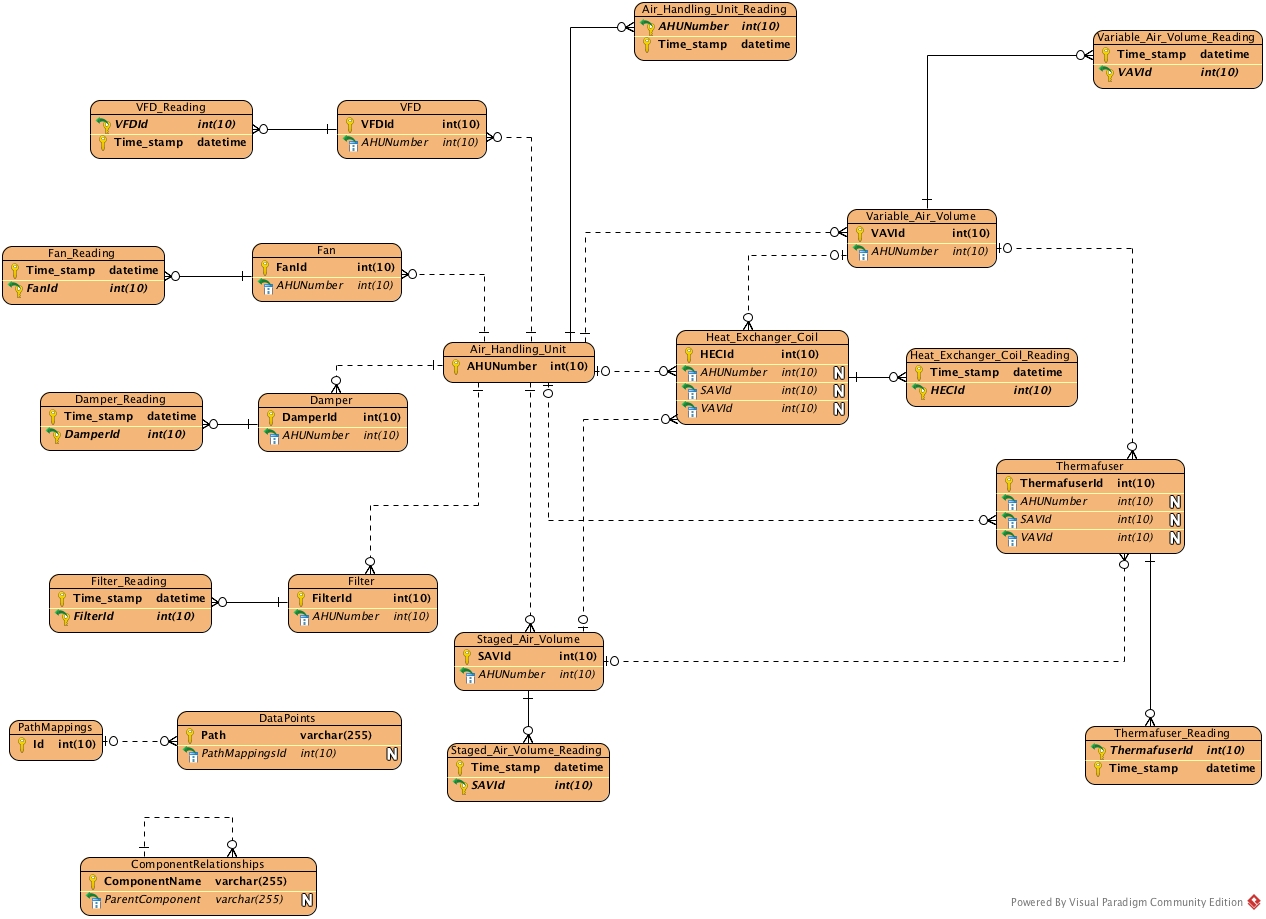
\includegraphics[width=150mm, height=100mm]{resources/HVAC_SE2_Names.jpg}
  	\caption{Proposed Database Design}
  	%\captionof{figure}{A figure}
 	\label{fig:databaseDesign}
\end{figure}

To save space only the tables, its primary and foreign keys and the relationships between tables are shown in Figure \ref{fig:databaseDesign}. The specific attributes for each table can be found in the Appendix \ref{section:appendixA}. Next, a discussion of the structure of the database is presented. 

As can be observed in the diagram presented in Figure \ref{fig:databaseDesign}, the central element is the \gls{ahu} table. An \gls{ahu} can supply conditioned air to many \glspl{vav}/\glspl{sav} while a \gls{vav}/\gls{sav} can only be supplied air by a single \gls{ahu} (with one exception in the case of the SE 2 \gls{hvac} which will be addressed further), this relationship is modeled in the database as a one-to-many relationship between the \gls{ahu} table and the \glspl{vav}/\glspl{sav} tables.

Moving downwards in the hierarchy of the \gls{hvac} network we find \glspl{vav}/\glspl{sav}, this components are represented by its own tabled in the database. Each \gls{vav}/\gls{sav} can supply air to a number of thermafusers in the last level of the \gls{hvac} hierarchy, nevertheless a thermafuser can only be supplied air by a single \gls{vav}/\gls{sav}, once again, this represents a one-to-many relationship between the \glspl{vav}/\glspl{sav} tables and the thermafuser table.

As stated earlier, each one of the major components in the \gls{hvac} system (\glspl{ahu}, \glspl{vav}, \glspl{sav}) may be made up of some more basic components. In general, any of the major components can contain a number of fans, dampers, cooling and heating coils (generalized here as heat exchanger coils), filters and VFDs, each of these components is represented in the database by its own table. Notice here, that while a particular major component can contain many of these components a particular instance of such components can only belong to one and only one \gls{ahu}, this is again reflected as a one-to-many relationship between the major and the minor components in the database.

Finally, each one of the components of the system (major and minor) have a number of sensors that provide readings and measurements of certain variables pertinent to each device. For each device, its own readings are represented as a table (with the prefix ``Reading'' on the name of the table) where a device may have many reading but a particular set of readings can belong to only one component, once again, this is represented as a one-to-many relationship between the component and its readings in the database. For a  full description of the variables pertinent to each component please refer to Appendix \ref{section:appendixA}.

This database design not only allows for a more reliable and efficient storage of the raw data, but also will help make the fault localization more accurate, since once a fault is detected by analyzing the data, its location can be accurately given by means of the primary keys of each table and the relationships among tables.


%------------------------------------------------

%----------------------------------------------------------------------------------------
%	GLOSSARY
%----------------------------------------------------------------------------------------
%\cleardoublepage
%\phantomsection
\addcontentsline{toc}{section}{List of Acronyms}
\printglossaries


%----------------------------------------------------------------------------------------
%	REFERENCE LIST
%----------------------------------------------------------------------------------------

\addcontentsline{toc}{section}{References}
\bibliographystyle{unsrt}
\bibliography{reference_introAndData}

%----------------------------------------------------------------------------------------

%----------------------------------------------------------------------------------------
%	Appendices
%----------------------------------------------------------------------------------------
\pagebreak
\appendix
%\nopartblankpage
\appendixpage

%\begin{appendices}
%\renewcommand\sectionname{Appendix}
%\chapter{Some Appendix}
%The contents...
%Appendices
\section{Sensor readings for each of the components in the HVAC system}
\label{section:appendixA}

\subsection{HEC Readings}

This table describes the variables used for HEC readings

\begin{table}[!htb]
\centering
\begin{tabular}{| l r |}
	\hline
	\textbf{Sensor Name}           & \textbf{Type} \\ 
  	\hline
Supply Water Temperature & real \\
Return Water Temperature & real \\
Valve Opening Percentage & real \\
  	\hline
\end{tabular}
\caption{HEC Readings}
\label{table:hec_readings}
\end{table}

\subsection{Thermafuser Readings}

This table describes the variables used for Thermafuser readings

\begin{table}[!htb]
\centering
\begin{tabular}{| l r |}
	\hline
	\textbf{Sensor Name}           & \textbf{Type} \\ 
  	\hline
Room Occupied               & bit  \\
Zone Temperature            & real \\
Supply Air                  & real \\
Airflow Feedback            & real \\
CO2 Input                   & real \\
Max Airflow                 & real \\
Min Airflow                 & real \\
Unoccupied Heating Setpoint & real \\
Unoccupied Cooling Setpoint & real \\
Occupied Cooling Setpoint   & real \\
Occupied Heating Setpoint   & real \\
Terminal Load               & -   \\
  	\hline
\end{tabular}
\caption{Thermafuser Readings}
\label{table:thermafuser_readings}
\end{table}

\pagebreak

\subsection{AHU Readings}

This table describes the variables used for \gls{ahu} readings

\begin{table}[!htb]
\centering
\begin{tabular}{| l r |}
	\hline
	\textbf{Sensor Name}           & \textbf{Type} \\ 
  	\hline
  	Zone Temperature         & real      \\
Static Pressure          & real      \\
Return Air Temperature   & real      \\
Supply Air Temperature   & real      \\
Exhaust Air Temperature  & real      \\
Outside Air Temperature  & real      \\
Smoke Detector           & bit       \\
Outside CO2              & real      \\
Return Air CO2           & real      \\
Spare                    & real      \\
Hi Static                & bit       \\
Duct Static Pressure     & real      \\
Mixed Air Temperature    & real      \\
Outside Air CFM          & real      \\
CoolingRequest           & real      \\
Cooling Setpoint         & real      \\
Heating Request          & real      \\
Heating Setpoint         & real      \\
Economizer Setpoint      & real      \\
Occupied Mode            & bit       \\
Return Air CO2 Setpoint  & real      \\
Static Pressure Smoothed & real      \\
Static SP                & real      \\
Supply Air Setpoint      & real      \\
STReq                    & -         \\
StaticSP1                & -         \\
StaticSP2                & -        \\
  	\hline
\end{tabular}
\caption{AHU Readings}
\label{table:ahu_readings}
\end{table}

\pagebreak

\subsection{SAV Readings}

This table describes the variables used for \gls{sav} readings

\begin{table}[!htb]
\centering
\begin{tabular}{| l r |}
	\hline
	\textbf{Sensor Name}           & \textbf{Type} \\ 
  	\hline
  	Misc Spare Input         & real \\
Zone Temperature         & real \\
Discharge Temperature    & real \\
Misc Input               & bit  \\
Condensate Detector      & bit  \\
Valve Output Percentage  & real \\
GEX Damper Position      & real \\
CoolingRequest           & real \\
Cooling Setpoint         & real \\
Heating Request          & real \\
Heating Setpoint         & real \\
Damper Position          & real \\
Exhaust Airflow          & real \\
Supply Airflow           & real \\
Flow Difference          & real \\
Exhaust Airflow Setpoint & real \\
Cooling Percentage       & real \\
Heating Percentage       & real \\
CER Temprature           & real \\
Ht Request               & real \\
Cl Request               & real \\
  	\hline
\end{tabular}
\caption{SAV Readings}
\label{table:sav_readings}
\end{table}


\subsection{VAV Readings}

This table describes the variables used for \gls{vav} readings

\begin{table}[!htb]
\centering
\begin{tabular}{| l r |}
	\hline
	\textbf{Sensor Name}           & \textbf{Type} \\ 
  	\hline
  	Flow Input            & real \\
Misc Spare Input      & real \\
Zone Temperature      & real \\
Discharge Temperature & real \\
Condensate Detector   & bit  \\
Duct Static Pressure  & real \\
Zone CO2              & real \\
Damper Position       & real \\
Cooling Setpoint      & real \\
Heating Setpoint      & real \\
  	\hline
\end{tabular}
\caption{VAV Readings}
\label{table:vav_readings}
\end{table}


\subsection{Fan Readings}

This table describes the variables used for Fan readings

\begin{table}[!htb]
\centering
\begin{tabular}{| l r |}
	\hline
	\textbf{Sensor Name}           & \textbf{Type} \\ 
  	\hline
  	Fan Type               & bit  \\
Air Velocity Pressure  & real \\
VFD Speed              & real \\
Fan Status             & bit  \\
VFD Fault              & bit  \\
Hi Static Reset        & bit  \\
FA Return fan Shutdown & bit  \\
Fan VFD                & bit  \\
Isolation Dampers      & bit  \\
Fan SS                 & bit  \\
Air Velocity CFM       & -   \\
  	\hline
\end{tabular}
\caption{Fan Readings}
\label{table:fan_readings}
\end{table}


\subsection{Filter Readings}

This table describes the variables used for Filter readings

\begin{table}[!htb]
\centering
\begin{tabular}{| l r |}
	\hline
	\textbf{Sensor Name}           & \textbf{Type} \\ 
  	\hline
Difference Pressure & real \\
  	\hline
\end{tabular}
\caption{Filter Readings}
\label{table:filter_readings}
\end{table}


\subsection{Damper Readings}

This table describes the variables used for Damper readings

\begin{table}[!htb]
\centering
\begin{tabular}{| l r |}
	\hline
	\textbf{Sensor Name}           & \textbf{Type} \\ 
  	\hline
Input Voltage      & real \\
Opening Percentage & real \\
Isolation Damper   & bit \\
  	\hline
\end{tabular}
\caption{Damper Readings}
\label{table:damper_readings}
\end{table}
%\end{appendices}


\end{document}
